%
% integralprinzip.tex
%
% (c) 2020 Prof Dr Andreas Müller, Hochschule Rapperswil
%
\begin{frame}[fragile]
\frametitle{Integral $\rightarrow$ Gleichung}
\vspace{-15pt}
\begin{columns}[t]
\begin{column}{0.48\hsize}
\begin{block}{Prinzip}
$f(x)$ eine stetige Funktion in $[a,b]$ und
\[
\int_a^b f(x) h(x) \,dx = 0\quad \forall h
\]
dann ist $f(x)=0$
\end{block}
\uncover<2->{%
\begin{proof}[Beweis]
\begin{enumerate}
\item<3->
Annahme: $f(\bar{x}) \only<-6>{>}\ifthenelse{\boolean{presentation}}{\only<7->{<}}{} 0$
\item<4->
$f(x) \only<-6>{>}\ifthenelse{\boolean{presentation}}{\only<7->{<}}{} 0$ für $|x-\bar{x}|\le \varepsilon$
\item<5->
Wähle $h(x)$ mit $h(x) > 0$ für $|x-\bar{x}|<\varepsilon$, $f(x)=0$ sonst.
\item<6->
$\int_a^b f(x)h(x) \,dx \only<-6>{>}\ifthenelse{\boolean{presentation}}{\only<7->{<}}{} 0\; \Rightarrow $ Widerspruch!
\qedhere
\end{enumerate}
\end{proof}}
\end{column}
\begin{column}{0.48\hsize}
\begin{center}
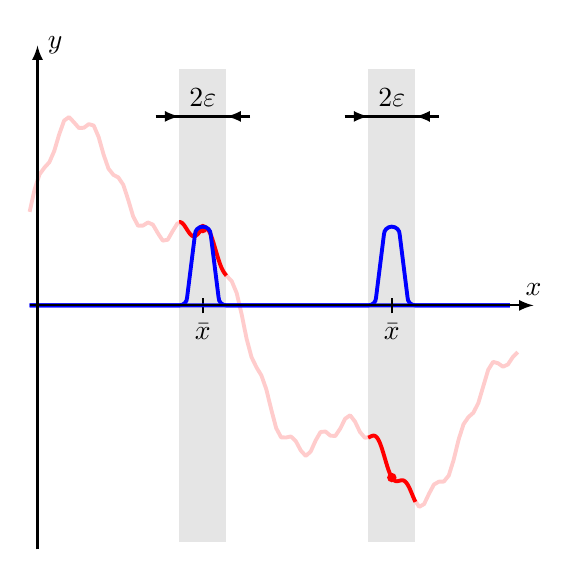
\begin{tikzpicture}[>=latex,thick]

\def\xzero{2.1}
\xdef\x{\xzero}
\pgfmathparse{0.5*sin(200*\x)+2.5*cos(47*\x)+2*sin(33*\x)+0.1*cos(1000*\x)-1}
\xdef\yzero{\pgfmathresult}

\def\xone{4.5}
\xdef\x{\xone}
\pgfmathparse{0.5*sin(200*\x)+2.5*cos(47*\x)+2*sin(33*\x)+0.1*cos(1000*\x)-1}
\xdef\yone{\pgfmathresult}

\def\hintergrund#1{
	\fill[color=gray!20] ({#1-0.3},-3) rectangle ({#1+0.3},3);
	\draw ({#1-0.4},2.4)--({#1+0.4},2.4);
	\draw[->] ({#1-0.6},2.4)--({#1-0.3},2.4);
	\draw[->] ({#1+0.6},2.4)--({#1+0.3},2.4);
	\node at (#1,2.4) [above] {$2\varepsilon$};
}

\uncover<5-6>{
	\hintergrund{\xzero}
}

\ifthenelse{\boolean{presentation}}{
\uncover<8->{
	\hintergrund{\xone}
}
}{}

\draw[color=red!20,line width=1.4pt,line join=round]
	plot[domain=-0.1:6.1,samples=100]
	({\x},{0.5*sin(200*\x)+2.5*cos(47*\x)+2*sin(33*\x)+0.1*cos(1000*\x)-1});

\uncover<4-6>{
	\draw[color=red,line width=1.4pt,line join=round]
	plot[domain={\xzero-0.3}:{\xzero+0.3},samples=100]
	({\x},{0.5*sin(200*\x)+2.5*cos(47*\x)+2*sin(33*\x)+0.1*cos(1000*\x)-1});
}

\uncover<3-6>{
	\fill[color=red] (\xzero,\yzero) circle[radius=0.06];
	\draw (\xzero,-0.1)--(\xzero,0.1);
	\node at (\xzero,-0.1) [below] {$\bar{x}$};
}

\uncover<5-6>{
	\draw[color=blue,line width=1.4pt,tension=0.1]
		(-0.1,0)
		-- ({\xzero-0.3},0)
		to[out=0,in=-90] ({\xzero-0.2},0.1)
		-- ({\xzero-0.1},0.9)
		to[out=90,in=180] (\xzero,1)
		to[out=0,in=90] ({\xzero+0.1},0.9)
		-- ({\xzero+0.2},0.1)
		to[out=-90,in=180] ({\xzero+0.3},0)
		-- (6,0);
}

\ifthenelse{\boolean{presentation}}{
\uncover<8->{
	\draw[color=red,line width=1.4pt,line join=round]
	plot[domain={\xone-0.3}:{\xone+0.3},samples=100]
	({\x},{0.5*sin(200*\x)+2.5*cos(47*\x)+2*sin(33*\x)+0.1*cos(1000*\x)-1});
}

\uncover<7->{
	\fill[color=red] (\xone,\yone) circle[radius=0.06];
	\draw (\xone,-0.1)--(\xone,0.1);
	\node at (\xone,-0.1) [below] {$\bar{x}$};
}

\uncover<9->{
	\draw[color=blue,line width=1.4pt,tension=0.1]
		(-0.1,0)
		-- ({\xone-0.3},0)
		to[out=0,in=-90] ({\xone-0.2},0.1)
		-- ({\xone-0.1},0.9)
		to[out=90,in=180] (\xone,1)
		to[out=0,in=90] ({\xone+0.1},0.9)
		-- ({\xone+0.2},0.1)
		to[out=-90,in=180] ({\xone+0.3},0)
		-- (6,0);
}
}{}


\draw[->] (-0.1,0)--(6.3,0) coordinate[label={$x$}];
\draw[->] (0,-3.1)--(0,3.3) coordinate[label={right:$y$}];

\end{tikzpicture}
\end{center}
\end{column}
\end{columns}
\end{frame}
